\section{My contribution}

\subsection{Introduction}

After outlining the context of the work-study program and describing the technique I worked
on, it is finally time to discuss my contributions to the project. First, I will explore 
the design I implemented and explain why this specific design was chosen. Next, we will 
examine the simulation models I developed and their applications. Following this, I will 
detail the optimization and parallelisation of the code that was done to enhance its performance. 
Finally, we will discuss how this optimized code could be utilised to estimate uncertainty
in real-time during synchrotron experiments.

\subsection{Design}

To gain a clear understanding of how this system works, let's visualize the design with the help of a 
UML diagram (see Figure \ref{fig:UML}). This diagram offers a roadmap, highlighting the various components and their interactions.
 We'll then delve deeper to explore each component's role in the system.
\subsubsection{Components}

\subsubsection*{\textbf{Fitter:}}
This class is a crucial component of the design. It includes the \textit{cmaes} function for estimating the
best-fit parameters and the \textit{mcmc} function for assessing the uncertainty in the fit. The class takes
a simulation model and experimental data as input. When the \textit{cmaes} function is called, it returns the best-fit parameters.
Subsequently, the \textit{mcmc} function can be invoked to provide statistical information about the best
fit, including the uncertainties in the parameters.

\subsubsection*{\textbf{Residual:}}
This class calculates the residuals between the experimental data and the model.
Currently, we use the log-likelihood as the residual function, but it can be easily extended
to other residual functions. The \textit{Fitter} class calls this class and provides the relevant model.
The \textit{Residual} class then uses the model's \textit{simulate\_diffraction} function to calculate
the model diffraction pattern and compare it with the experimental data.

\medskip

\begin{figure}[h]
    \centering
    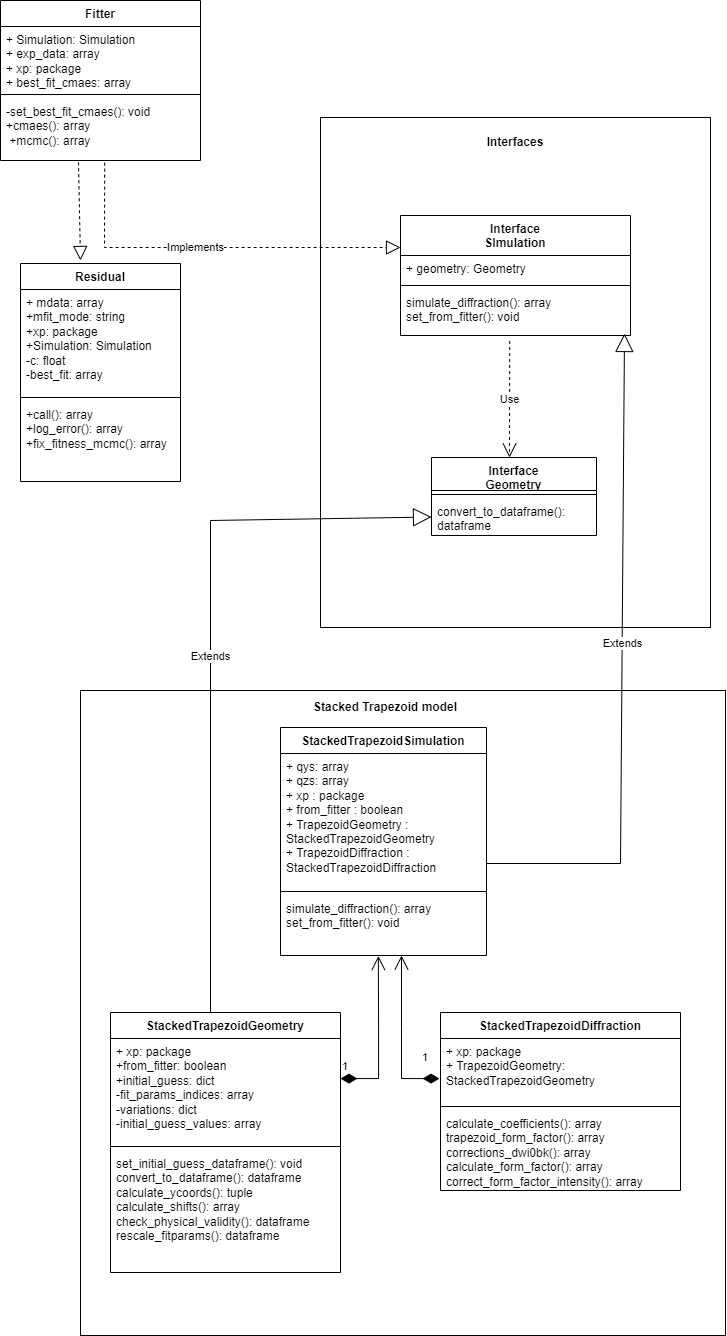
\includegraphics[width=0.7\textwidth]{images/cdsaxs_UML.png}
    \caption{UML diagram of the design for CD-SAXS simulation application. }
    \label{fig:UML}
\end{figure}

\FloatBarrier

\subsubsection*{\textbf{Simulation interface:}}

This is the base class for all simulation models. The functions and classes used in it should be implemented
in all simulation models.

\subsubsection*{\textbf{Geometry interface:}}

Like Simulation interface. This is the base class for all geometry models.


\subsubsection*{\textbf{Model:}}

In this UML diagram (Figure \ref{fig:UML}), we present the implementation of the stacked trapezoid model.
 Central to this model is the \textit{StackedTrapezoidSimulation} class, which is a composite class 
 integrating \textit{StackedTrapezoidGeometry} and \textit{StackedTrapezoidDiffraction} classes. The 
 \textit{StackedTrapezoidGeometry} class handles all geometrical calculations and stores the relevant 
 information, while the \textit{StackedTrapezoidDiffraction} class is responsible for all diffraction-related 
 calculations.

 \medskip

These classes work together to simulate the physics and generate data that can be compared with experimental
results. Throughout the project, additional models are being developed and they will be discussed later. The stacked 
trapezoid model serves as a prototype, illustrating how other models will be implemented. Each model will 
adhere to the base interfaces \textit{Simulation} and \textit{Geometry}.

\subsubsection{Relationships between components}

\medskip

This system is designed to simulate and analyze diffraction patterns using
 a modular approach. At its core, the system comprises several key components:
  the \textit{Fitter}, \textit{Residual}, and interfaces for \textit{Simulation}
   and \textit{Geometry}, along with specific model implementations like the
   \textit{StackedTrapezoidSimulation}. The \textit{Fitter} class orchestrates
the fitting process by using the \textit{cmaes} function to estimate the best-fit parameters and
 the \textit{mcmc} function to assess the uncertainty in the fit. It takes in a model and
  experimental data, utilising the \textit{Residual} class to compute the difference between
   the experimental data and the model's simulated data. The \textit{Residual} class leverages
    the model's \textit{simulate\_diffraction} function to generate the diffraction pattern,
     which it then compares with the experimental data.

\medskip

The model, meaning specific implementations of the interfaces, is designed to operate 
independently, allowing users to utilize a particular model
for simulations without needing to engage with the fitting component. This autonomous 
functionality ensures that users can easily perform simulations solely with the model of
 their choice. This design choice enhances flexibility and usability, as it decouples the simulation process from the fitting procedures, making it more accessible for users who may only need to run simulations.
The usefulness and implications of this design choice will be discussed shortly.


\subsubsection{Why this design?}
Let's first discuss the shortcomings of the previous design before explaining why the current design was chosen.

\subsubsection*{Previous design:}

The previous design adopted a monolithic approach, where the fitting and simulation components were tightly coupled. This meant that any changes to the fitting algorithm (e.g., adding a new optimization technique) would necessitate modifications to the simulation code as well. This interdependence made it difficult to introduce new functionalities or modify existing ones without potentially impacting other parts of the system.

\medskip

\begin{figure}[h]
    \centering
    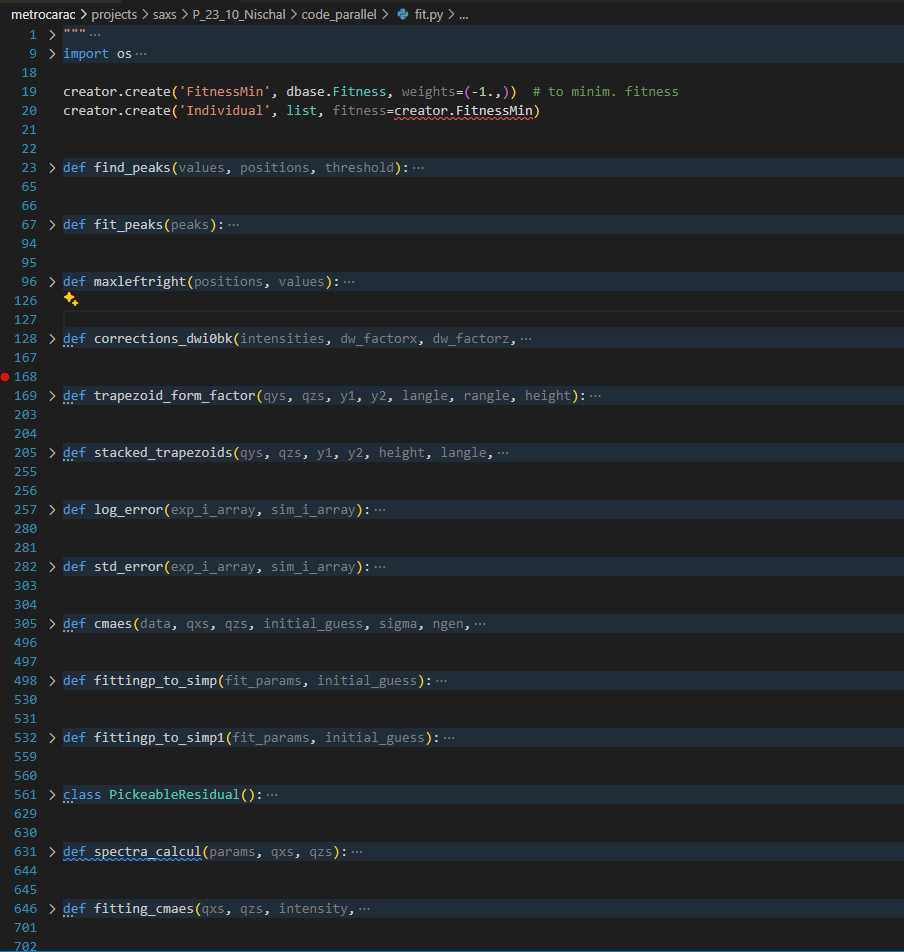
\includegraphics[width=0.5\textwidth]{images/monolithic.png}
    \caption{Monolithic design of the previous version. This script combined all the functions for the stacked trapezoid model
     in one file.}
    \label{fig:monolithic_design}
\end{figure}

Furthermore, individual models within the system implemented their own fitting and simulation functionalities. This resulted in a 
significant amount of code duplication, leading to inconsistencies between models. Moreover, adding new models required rewriting 
these functionalities from scratch, hindering the system's scalability. This approach proved inefficient for managing a growing number 
of models. These two limitations combined made it challenging to optimize or parallelize the code effectively. Since the fitting and 
simulation components were intertwined, it was difficult to isolate and optimize individual sections for improved performance.

\medskip

Similarly the codes for the different models each implemented their own fitting and simulation
components, leading to code duplication and inconsistencies across models. This design was not
scalable, as adding new models required rewriting the fitting and simulation components for each
model.

\subsubsection*{Current design:}

The current design improves upon the previous version by decoupling the fitting and 
simulation components, resulting in a modular structure. The \textit{Simulation} interface serves
 as the connecter between fitting and simulation, standardizing the process of fitting 
 any model.

\medskip

Also, by enabling simulation models to be developed independently of the fitting component, 
new models can be introduced without modifying the existing codebase. Developers can 
focus on developing new models without concerning themselves with the fitting process. 
This design choice significantly enhances the system's flexibility and scalability.

\medskip

The decoupling of components also facilitates optimization and 
parallelisation by allowing developers to focus on specific areas of improvement without
cross-component interference. For example, the simulation component can be optimized to
run faster and more efficiently through advanced numerical methods and parallel 
computing techniques. This is particularly beneficial for handling large datasets or complex simulations that demand significant 
computational resources. By isolating the simulation component, developers can experiment with and implement various optimization strategies, 
ensuring that the component runs as efficiently as possible.

\medskip

\subsection{Simulation Models}

In the realm of nano scale fabrication, techniques like photoresist lithography stands out as a pivotal technique. To model the structures 
resulting from photoresist lithography, we can observe that many of these structures can be approximated by stacked trapezoids. 
This simplification forms the foundation of our modeling approach. By considering the cross-sectional shapes of these lines, which 
closely resemble trapezoids, we can create computational models that simulate the fabrication process and predict the resulting 
geometries.

\medskip

Our models aims to balance accuracy and computational efficiency. While real structures are complex and not perfectly trapezoidal, 
using a series of stacked trapezoids provides a practical approximation that can be refined as needed. This approach serves as a robust
starting point for simulations, allowing us to incrementally increase the number of trapezoids to better match the real structures.

\medskip

Furthermore, we extend this model to account for rounded corners, which are common in actual fabricated structures. By approximating 
these rounded corners with smaller trapezoids, we can enhance the accuracy of our simulations without significantly increasing 
computational costs. Future developments may explore more direct modeling techniques, such as using sections of circles, to further
improve the fidelity of our models.

\medskip

Lastly, we introduce the overlay model, which simulates the alignment of different layers on a wafer.


\subsubsection{Brief overview of photoresist lithography}

These models are build to simulate the simple structure obtained through techniques like photoresist 
lithography. It is a technique used to fabricate micro and nano scale structures on substrates. 
It works by first coating the wafer with a light-sensitive material called photoresist. Then, a patterned
 mask blocks light from specific regions of the photoresist. 
 \begin{figure}[h]
    \centering
    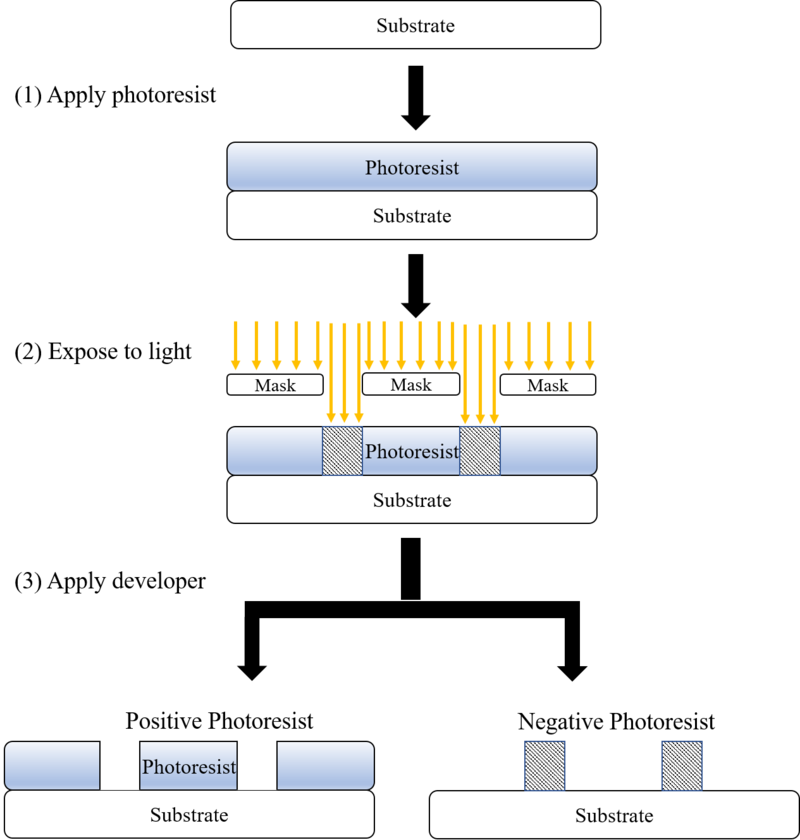
\includegraphics[width=0.4\textwidth]{images/photo_resist.png}
    \caption{Schematic of the photoresist lithography process (taken from wikipedia).}
    \label{fig:lithography}
 \end{figure}

 \FloatBarrier

 Exposing the wafer to light triggers a 
 chemical change in the exposed photoresist, making it either soluble (positive tone) or insoluble 
 (negative tone) in a developer solution. This developer removes the unwanted photoresist, 
 revealing the desired circuit pattern on the underlying wafer. Optionally, etching can be used to 
 create physical features by removing exposed areas of the substrate.

 \medskip

While developing our model, we consider lines of nanostructures on a substrate (see figure \ref{fig:lines}) obtained through this process.

\begin{figure}[h]
    \centering
    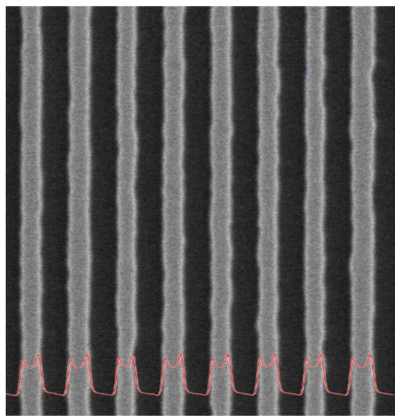
\includegraphics[width=0.3\textwidth]{images/lines_modeled.png}
    \caption{Image obtained with a scanning electron microscope in 
      top view of the structure for modelling. In red, the average signal over the length of the lines is superimposed.\cite{these_reche}}
    \label{fig:lines}
\end{figure}

\subsubsection{Stacked Trapezoid Model}

A close examination of the cross-section of the lines in Figure \ref{fig:lines} reveals that their shapes can be closely approximated by stacked trapezoids. This crucial observation forms the foundation of our modeling approach.

\medskip

\begin{figure}[h]
    \centering
    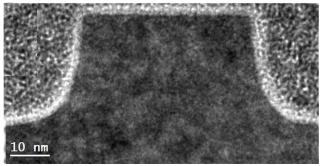
\includegraphics[width=0.4\textwidth]{images/trap_model.PNG}
    \caption{Tunneling electron microscope image of the cross section of the lines.\cite{phd_freychet}}
    \label{fig:trapezoid}
\end{figure}

Figure \ref{fig:trapezoid_model} illustrates the approximation of the model we aim to simulate. 
The model inputs include a constant height or sets of heights, sidewall angles ($\beta$), and the
 bottom width of the trapezoids. By allowing variable heights for each trapezoid layer, we can 
 achieve better control over the structure, albeit at the cost of increasing the number of 
 parameters to fit. The user can determine the height parameter based on their specific needs. 
 Given the z-coordinates of each corner of the trapezoids, the x-coordinate for each can be 
 calculated using the following formula:

\medskip

\begin{equation}
    x_{i} = x_{i-1} + \frac{z_{i} - z_{i-1}}{\tan(\beta)}
\end{equation}

\medskip

As discussed in Section \ref{sec:scattering_model}, we can use Equation \ref{eq:trapezoidal_ft} 
to calculate the Fourier transform of a single trapezoid and then sum them all up of 
all the trapezoids to obtain the diffraction pattern.

\medskip

This model has its limitations, as it simplifies the real structure. The actual structure is more 
complex and does not consist of perfect trapezoids. Additionally, a more detailed model would 
entail higher computational costs. Therefore, a balance between accuracy and computational cost 
is necessary. Despite these limitations, this model provides a solid foundation for simulations. 
By increasing the number of trapezoids, we can approximate the real structure more closely. Future
models will inherit from or build upon the \textit{StackedTrapezoidSimulation} and 
\textit{StackedTrapezoidGeometry} classes.

\medskip

\subsubsection{Rounded corners model}

The rounded corners model is an extension of the stacked trapezoid model. It is designed to 
simulate the rounded corners often found in real structures (see Figure \ref{fig:trapezoid}). 
Each corner of the trapezoid is rounded using a circle, with the radius of each circle provided 
as an input by the user and fitted later. Once the radii are known, the corners are approximated 
by dividing them into even smaller trapezoids. This allows us to use the same diffraction code written for the
 stacked trapezoid model to simulate the rounded corners. With this model, we can simulate the 
 diffraction pattern more accurately, reflecting the real structure more closely.

\begin{figure}[h]
    \centering
    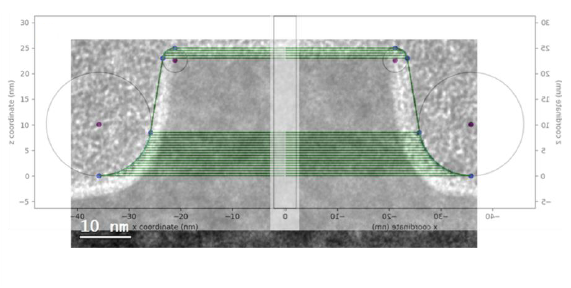
\includegraphics[width=0.8\textwidth]{images/rounded.PNG}
    \caption{Rounded corners model fitted on top of the scanning electron microscope image. (Image taken from the Work-study project report of Timothee Choisinet.) }
    \label{fig:rounded_corners}
\end{figure}

\medskip

While this model hasn't been implemented yet, a similar codebase already exists. This existing
code provides a strong foundation, potentially making implementation a smoother process.

\medskip

Simulating rounded corners with a large number of trapezoids significantly increases the 
computational cost of the model. To address this, exploring alternative approaches for representing 
rounded corners is a promising avenue for future development. One potential solution lies in 
directly incorporating a section of a circle into the model. This could involve calculating the 
direct Fourier transform of the circular segment and then summing the resulting components to obtain the 
diffraction pattern. This method has the potential to significantly reduce the computational 
complexity compared to using a multitude of trapezoids.

\subsubsection{Overlay model}

Silicon wafers are built layer-by-layer through a series of steps called photolithography. 
Each layer involves depositing a specific material (like a metal for contacts or a 
special material for transistors) in a defined pattern. Precise alignment between these 
layers is crucial for the final device to function properly. This means features like 
contacts, lines, and transistors must be perfectly positioned relative to each other 
on the wafer.

\medskip

\begin{figure}[h]
    \centering
    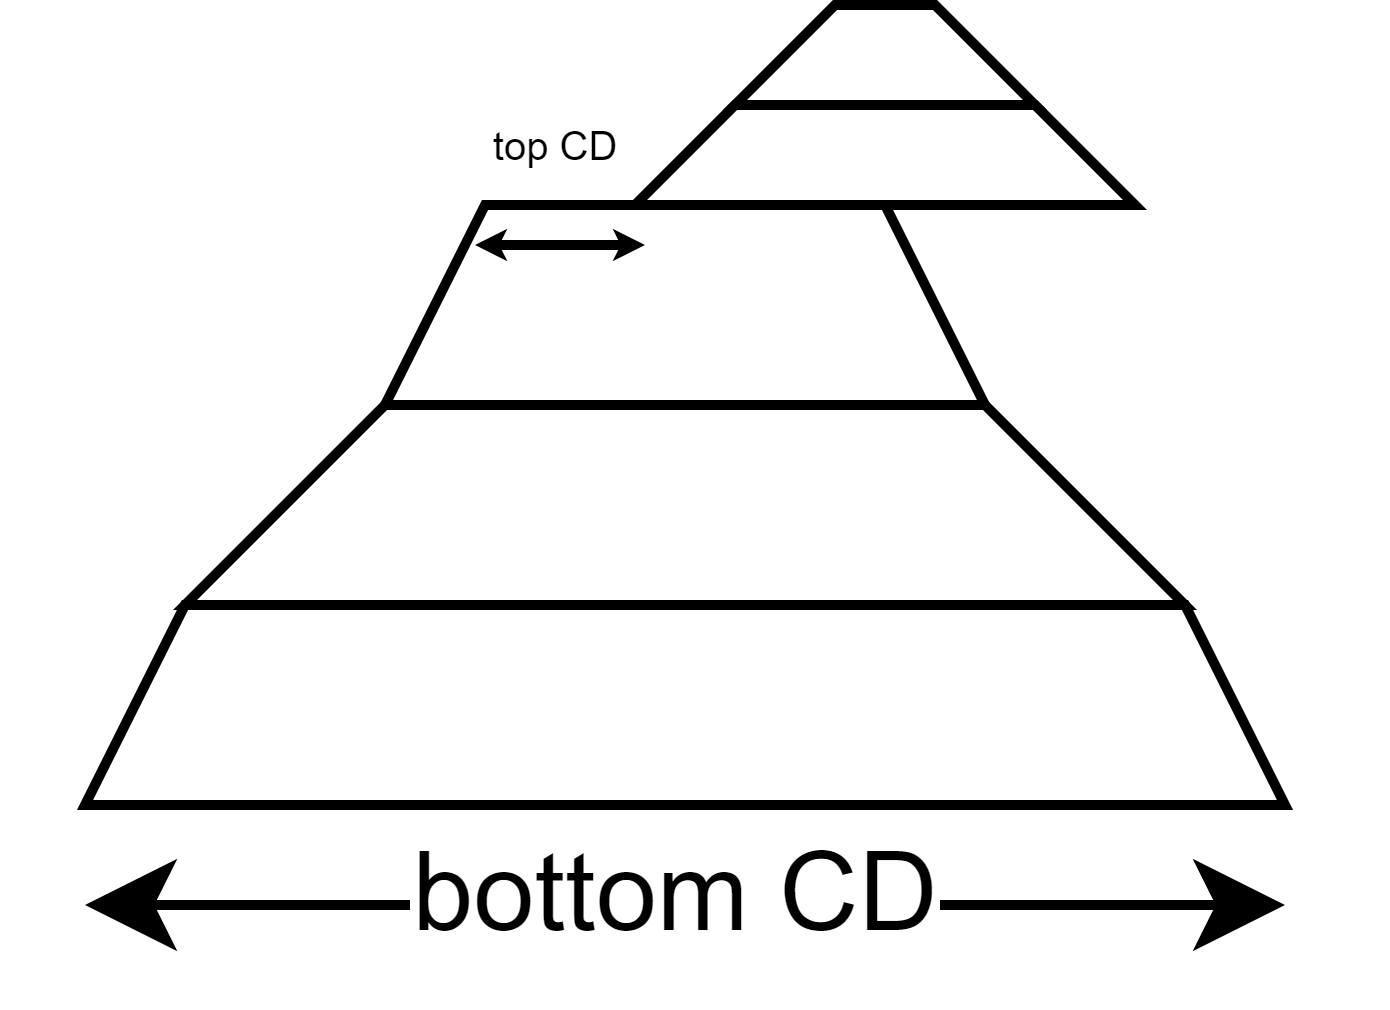
\includegraphics[width=0.5\textwidth]{images/overlay.PNG}
    \caption{Overlay model.}
    \label{fig:overlay}
\end{figure}

\FloatBarrier

The overlay model is designed to simulate the critical aspect of layer alignment during wafer 
fabrication. This model builds upon the concept of the stacked trapezoid model, but extends it to 
capture misalignment effects. It incorporates two sets of trapezoids: one set for each layer. The 
key difference lies in the positioning of the second layer's trapezoids. These are shifted by a 
specific amount, called the Top Critical Dimension (Top CD), in the x-direction. This shift 
represents potential misalignment between layers.

\medskip

To calculate the coordinates of the second layer's trapezoids, we can leverage the same method 
used for the stacked trapezoid model. However, for the second layer, an additional x-axis shift 
equal to the Top CD value is applied.

\medskip

To add the overlay model to the code, we inherit from the \textit{StackedTrapezoidSimulation} and \textit{StackedTrapezoidGeometry} classes.
The \textit{StackedTrapezoidGeometry} class will be modified to include the shift in the x direction for the second layer. This shift is entered by the
user and is fitted later on.

\subsection{Implementation of MCMC to Measure Uncertainty}

As discussed in Section \ref{sec:mcmc_cdsaxs}, after finding the best fit for a model using the \textit{cmaes} algorithm, it is crucial 
to determine the uncertainty in the fitted parameters. This is where the \textit{mcmc} method of the \textit{Fitter} class becomes essential. 
While we follow a similar approach to the algorithm described in Section \ref{sec:mcmc_cdsaxs}, there are key differences that will be discussed 
in this section, along with the method's implementation and its outputs.

\medskip

We utilize the \textit{emcee} Python package \cite{emcee} to implement this method. This package is well-regarded for its ease 
of use and effective implementation of the MCMC algorithm, having been referenced in several scientific papers \cite{emcee_refed}. 
A significant advantage of \textit{emcee} is the flexibility it offers in choosing the type of moves for the MCMC algorithm. Unlike 
the Metropolis-Hastings criterion used in Section \ref{sec:mcmc_cdsaxs}, \textit{emcee} employs the stretch move by default, which 
has been shown to achieve faster convergence \cite{goodman2010_strech_move,emcee}. The stretch move uses the following formula to 
determine whether to accept or reject a move:

\begin{equation}
    P_{i} = e^{Z^{1-N} (GF_{i} -GFB)}
\end{equation}

where \(P_{i}\) is the probability of accepting the move, \(N\) is the number of parameters, \(GF_{i}\) is the current goodness of fit, 
and \(GFB\) is the goodness of fit of the initial fit. \(Z\) is drawn randomly from the distribution:

\begin{equation}
    Z \in g(z) \propto 
    \begin{cases} 
      \frac{1}{z} & \text{for } z \in \left[\frac{1}{a}, a\right] \\
      0 & \text{otherwise}
    \end{cases}
\end{equation}

\medskip

In addition, \textit{emcee} includes a built-in function to calculate the autocorrelation time of the chain, which helps determine which part of the chain to use for statistical analysis. We implemented the \textit{mcmc} method using the default stretch move of \textit{emcee}, but also provided options to use other moves like Metropolis-Hastings and Gaussian moves.

\medskip

For the implementation, the user needs to provide the following inputs:
\begin{itemize}
    \item The number of parameters
    \item $\sigma$, which is the standard deviation of the initial walker population
    \item The number of steps to run the MCMC algorithm
    \item The number of walkers
    \item A directory to save the statistical analysis information(optional)
\end{itemize}

\medskip

Unlike previous approaches \cite{sunday2016evaluation}, we do not vary the model parameters directly.
 Instead, we use a normalized space where variations range between $-\sigma$ and $\sigma$. These 
 normalized values are then rescaled to the actual parameter values using the following formula:

\begin{equation}
    \text{Rescaled Params} = \text{Normalized Params} \times \text{Allowed Range} + \text{Best Fit Cmaes}
\end{equation}

This approach provides better control over the parameter range, preventing unnecessary exploration of 
regions far from the best fit. It also allows the best fit obtained from the CMAES algorithm to serve as the mean of the initial walker population.

\medskip

After extracting the chain from the MCMC algorithm, we perform a statistical analysis. This includes calculating 
the mean, standard deviation, total number of individuals in the chain, minimum and maximum parameter values, lower
 and upper confidence intervals as specified by the user, and the uncertainty in the parameters, defined as the difference between the upper and lower confidence intervals.

\begin{figure}[h]
    \centering
    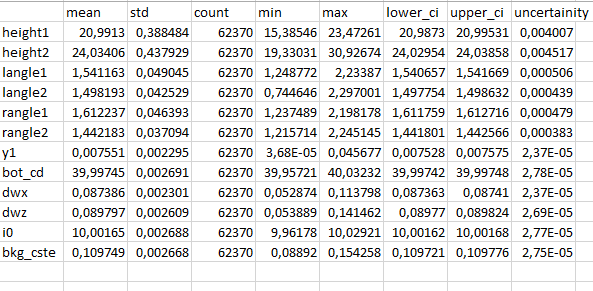
\includegraphics[width=0.8\textwidth]{images/mcmc_out.png}
    \caption{Example of output statistics file of the MCMC algorithm. The model used was the stacked trapezoid model.}
\end{figure}

\FloatBarrier

In conclusion, the implementation of the MCMC method using the \textit{emcee} package has proven to be an effective
approach for quantifying the uncertainty in the parameters of our models. By leveraging the flexibility and advanced
features of \textit{emcee}, such as the stretch move and autocorrelation time calculation, we have enhanced the robustness
and efficiency of our statistical analysis. The normalization and rescaling strategy we employed allows for better
control over the parameter space, ensuring a more focused exploration around the best fit obtained from the CMAES
algorithm. This method not only provides detailed statistical insights into the model parameters but also sets 
a solid foundation for future improvements and extensions. The versatility and precision of the MCMC method make 
it a valuable tool in the continuous effort to refine our simulations and better understand the underlying physical structures.


\subsection{Parallelisation and GPU Acceleration}

The simulation of diffraction patterns can be computationally intensive, especially when dealing with large datasets or complex models. 
Given that the code is written in Python, which is inherently slower than compiled languages like C++, optimizing for performance is crucial. 
One effective strategy for improving performance is parallelisation. By distributing the computational workload across multiple cores or processors, 
we can significantly reduce simulation time. In this section, we will briefly discuss parallelisation and overview the strategies for parallelisation 
on both GPU and CPU.

\medskip

\subsubsection{Overview of Parallelisation}

Parallelisation involves breaking down tasks into independent units. Instead of performing a complex calculation in one go, the task is 
distributed across multiple processors for simultaneous processing. This approach leverages the power of modern hardware, with multiple cores 
on a single processor or distributed computing systems. The key is to achieve the right balance: tasks must be independent to avoid communication 
overhead yet large enough for efficient processing. While challenges exist, such as managing communication and limited parallelizability for certain 
problems, parallelisation is a game-changer in fields like scientific computing, machine learning, and video processing.

\medskip

If we can use the GPU to perform calculations in parallel, we can achieve a significant speedup. However, there is a catch: the GPU is not as 
flexible as the CPU. It is designed for parallel processing of large amounts of data, making it ideal for tasks like matrix multiplication. However, 
the GPU is not well-suited for tasks that require branching or recursion, as these can slow down processing speed. Therefore, to take full advantage of 
the GPU, we need to structure our code in a way that aligns with the GPU's strengths.

\medskip

\begin{figure}[h]
    \centering
    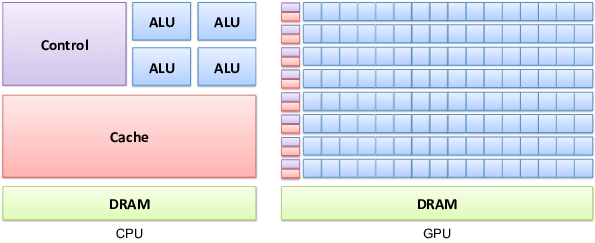
\includegraphics[width=0.8\textwidth]{images/gpu_vs_cpu.png}
    \caption{Comparison between GPU and CPU. The GPU has more cores but is less flexible than the CPU, making it suitable for simpler parallel tasks. \cite{gpu_vs_cpu}}
\end{figure}

\subsubsection{Parallelisation Strategies}

To parallelize the code, we need to identify the independent parts. In both the \textit{cmaes} and \textit{mcmc} algorithms, a population is generated 
for each generation (or step), and each individual in the population is evaluated independently to calculate the goodness of fit. Since one generation 
depends on the best fit of the previous generation, parallelizing the generation is not possible. However, parallelizing the evaluation of individuals 
in the population is possible.

\medskip

Initially, to avoid the complexity of GPU parallelisation, we used the multiprocessing library in Python to parallelize the code. This library allows 
us to run multiple processes in parallel, each on a different core. We used the \textit{Pool} class from the multiprocessing library to create a pool 
of workers, each evaluating the goodness of fit. This approach reduced computation time significantly, as multiple individuals could be evaluated simultaneously.

\medskip

However, the code still contained many for-loops that could be parallelized using NumPy operations. NumPy, being a highly optimized library for numerical 
operations, was used to further optimize the code. Wherever for-loops could be replaced by NumPy operations, we did so, further reducing computation time. 
The major challenge was that the quantities we wanted to perform operations on were not of the same shape, requiring the use of NumPy broadcasting to 
perform the operations (see Figure \ref{fig:broadcasting} for an example).

\medskip

\begin{figure}[h]
    \centering
    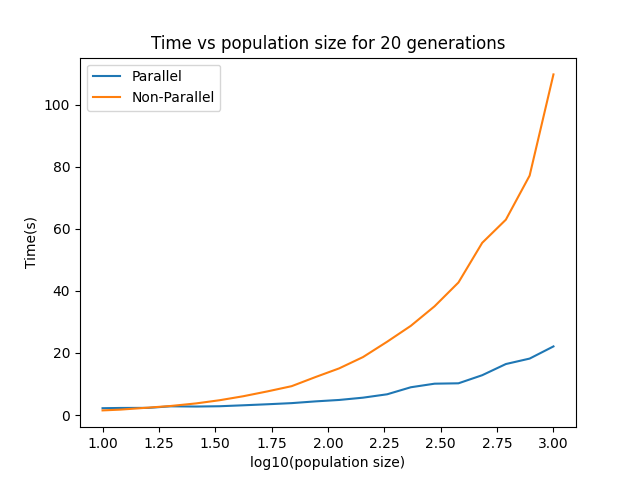
\includegraphics[width=0.7\textwidth]{images/multiprocessing.png}
    \caption{Multiprocessing used to improve the execution time of the code for the \textit{cmaes} algorithm. The generation was fixed to 20.}
\end{figure}

\begin{figure}[h]
    \centering
    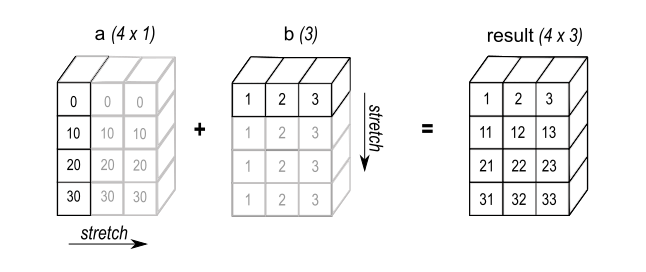
\includegraphics[width=0.7\textwidth]{images/broadcasting.png}
    \caption{NumPy broadcasting used to perform operations on arrays of different shapes (image taken from NumPy documentation).}
    \label{fig:broadcasting}
\end{figure}

\FloatBarrier

After this step, it was easier to parallelize the code for GPU. As the code was already vectorized, we used the CuPy library, a GPU-accelerated 
version of NumPy. CuPy is built on top of CUDA, a parallel computing platform and application programming interface created by Nvidia. CuPy uses 
CUDA libraries like cuBLAS, cuDNN, cuFFT, cuSPARSE, etc., which are highly optimized for parallel computing (more information can be found in its 
documentation page \cite{cupy}).

\begin{figure}[h]
    \centering
    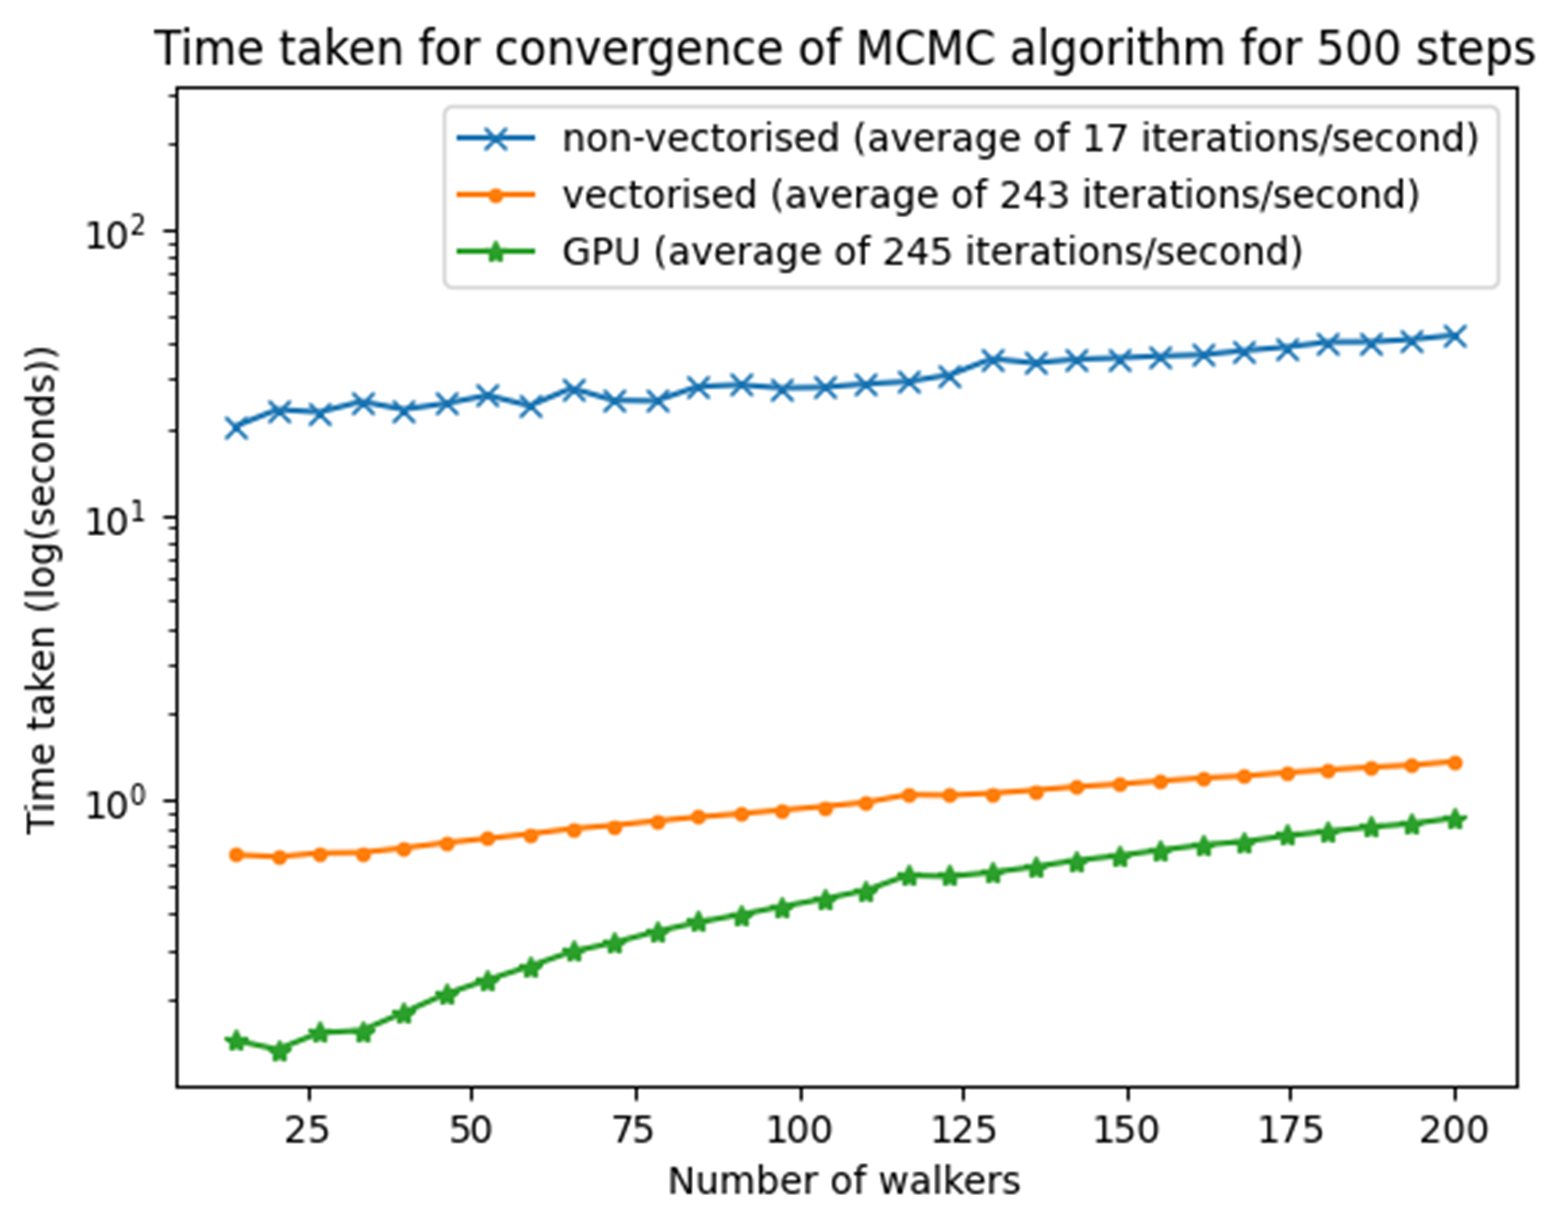
\includegraphics[width=0.8\textwidth]{images/gpu.png}
    \caption{CuPy used to parallelize the code. The number of iterations per second in the parallel version is much higher. (This test was performed 
    on CEA aar164 server Intel(R) Xeon(R) Platinum 8362 CPU @ 2.80GHz, 128 cores, and NVIDIA A100 80GB GPU)}
    \label{fig:cupy}
\end{figure}

\FloatBarrier

However, we are essentially replacing NumPy operations with CuPy operations, some operations 
are more efficient in NumPy than in CuPy. For example, cumulative sum in CuPy is slower than in 
NumPy because the nature of the operation is not parallelizable. However, the calculation of the 
analytical Fourier transform and the calculation of log error are much faster in CuPy than in 
NumPy. Thus, we still need to identify the parts of the code that are slowing down the execution 
time due to communication overhead and replace them with NumPy operations. This is perhaps why 
we don't see a significant speedup in the execution time in Figure \ref{fig:cupy}. However, the 
code is now ready to be used on a GPU and can be further optimized. This will be the next step 
in the project.

\medskip

In conclusion, parallelisation and GPU acceleration have significantly enhanced the performance
 of our diffraction pattern simulation and fitting code. By leveraging the multiprocessing 
 library and NumPy optimizations, we achieved considerable speedups in CPU-based parallelisation. 
 Transitioning to GPU parallelisation using CuPy further improved execution times, although some
  operations still perform better in NumPy due to their non-parallelizable nature. Future work 
  will focus on identifying and optimizing these bottlenecks to fully harness the power of GPU 
  acceleration. The groundwork laid here provides a robust foundation for further improvements 
  and scalability in our computational simulations.


  \subsection{On-the-Fly Uncertainty Estimation}

  Another objective identified in our research was to utilize the code to estimate 
  uncertainty in real-time during synchrotron experiments. The uncertainty in CD-SAXS experiments 
  depends on various factors such as exposure time, sample thickness, detector distance, etc. Among 
  these, exposure time plays a crucial role in determining uncertainty. The study by Sunday et al. \cite{sunday2016evaluation} 
  provides an excellent example of this relationship (see Figure \ref{fig:exposure}).
  
  \begin{figure}[h]
  \centering
  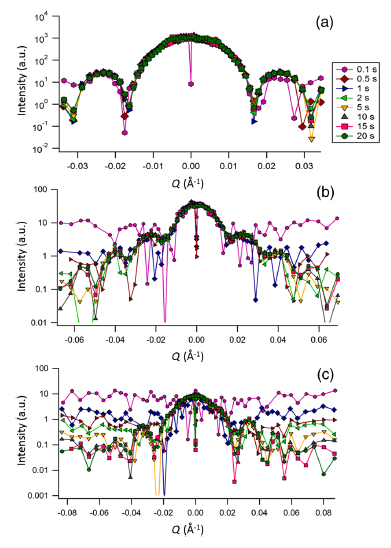
\includegraphics[width=0.4\textwidth]{images/exposure.png}
  \caption{Uncertainty in fit parameters as a function of exposure time. The uncertainty decreases with increasing exposure time. (Sunday et al. \cite{sunday2016evaluation})}
  \label{fig:exposure}
  \end{figure}
  
  Sunday et al. conducted measurements over a range of angles with specified step sizes for different 
  acquisition times. Their results, shown in the figure, present representative data cuts for various 
  order peaks, illustrating the impact of exposure time on data quality. The first-order peak, which 
  exhibits the most intense scattering, remains well-defined even at shorter acquisition times. However, 
  as the measurement time decreases, the lower intensity features of the higher-order peaks become 
  progressively obscured due to the decreasing signal-to-noise ratio.
  
  If we could estimate uncertainty in real-time during the experiment, it would enable us to adjust 
  various parameters including exposure time affecting uncertainty on the fly. Additionally, we could stop the experiment 
  after measuring a sufficient number of angles. The same paper by Sunday et al. demonstrates that 
  beyond a certain number of angles, the uncertainty does not change significantly. This approach 
  could facilitate performing CD-SAXS experiments in laboratory settings with equipment less powerful 
  than synchrotrons.
  
  To investigate this, a simulation was conducted using the stacked trapezoid model. A two-stack 
  trapezoid was considered with the following parameters: \( h_{1} = h_{2} = 21.5 \) nm, bottom CD = 24 nm, 
  first sidewall angle = 85°, and second sidewall angle = 90°. The simulation aimed to mimic 
  data acquisition at different angles with a measurement time of 2 seconds per angle. The uncertainty 
  was calculated after every 15 angles measured. The results are shown in Figure \ref{fig:uncertainity}.

  \begin{figure}[h]
  \centering
  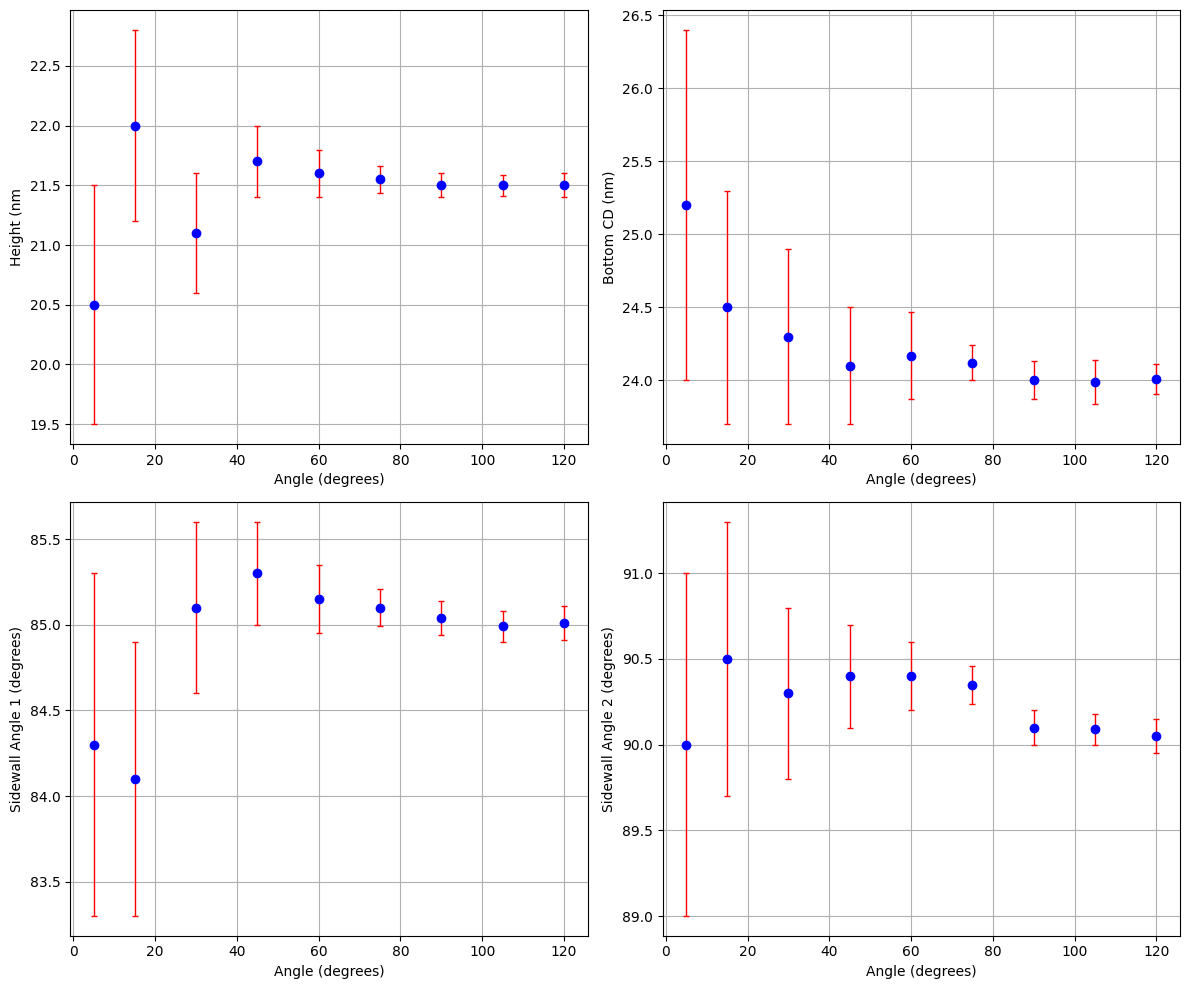
\includegraphics[width=0.8\textwidth]{images/uncertainity.png}
  \caption{Uncertainty in the fit parameters as a function of the number of angles measured.}
  \label{fig:uncertainity}
  \end{figure}
  
  As seen in Figure \ref{fig:uncertainity}, the uncertainty levels off after a certain number of angles, similar to the findings by Sunday et al.
   However, in our simulation, the angle at which uncertainty stabilizes is around 78 degrees, 
   compared to 30 degrees in their study. This discrepancy could be due to differences in the measured
structures and other factors. Nevertheless, this simulation demonstrates the feasibility of real-time 
uncertainty estimation during experiments, allowing for parameter adjustments as needed. Further 
testing with extensive real data is necessary to validate this approach, which is an ongoing effort.
